\documentclass{article}
\usepackage[utf8]{inputenc}

\title{Lesson 5 - Computer Organization}
\author{Matt Chung}
\date{July 27 2017}
\usepackage{amsfonts}
\usepackage{ulem}
\usepackage{amsmath}
\usepackage{graphicx} 
\renewcommand{\thesubsection}{\thesection.\alph{subsection}}

\begin{document}

\maketitle

\section{}
% https://tex.stackexchange.com/questions/32886/how-to-fit-a-large-figure-to-page
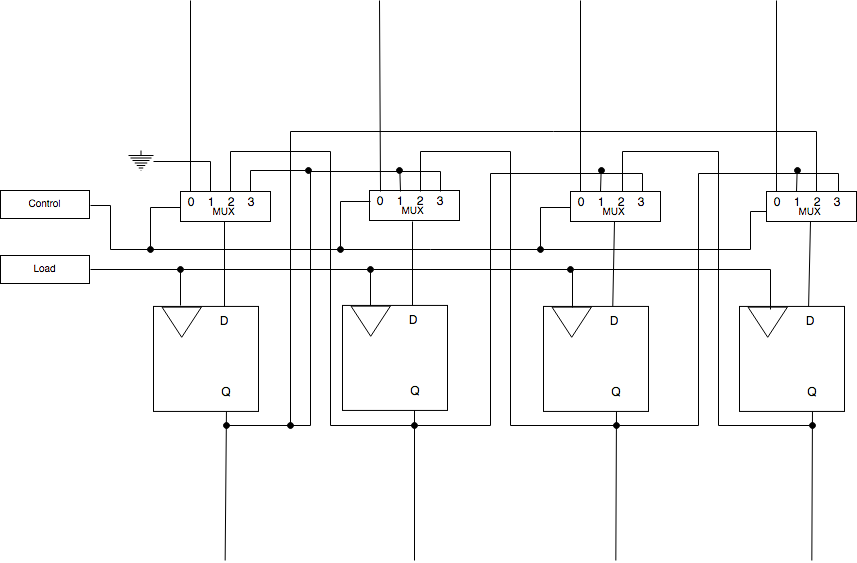
\includegraphics[width=\textwidth, height=\textheight, keepaspectratio]{q1}

\section{}
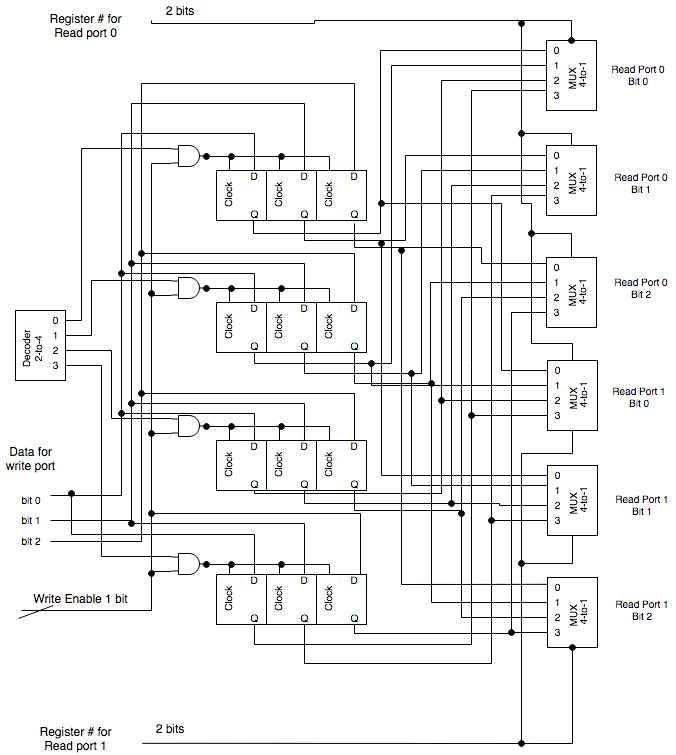
\includegraphics[width=\textwidth, height=\textheight, keepaspectratio]{lesson-5-question-2}

\section{}
Despite the drawback of requiring to be refreshed, dynamic RAM (capacitor based) has an advantage over static memory (SR-latch based) when storing a single bit. Static memory requires four gates: (2) NOR and (2) AND gates. On the other hand, dynamic ram only requires a single capacitor, allowing us to add four times as much capacity. Of course, there's a drawback: dynamic ram runs a bit slower, requiring to be refreshed, adding some latency to detect the voltage. But this reduced performance is marginal compared to the increased capacity.

\section{}

Although main memory can be implemented with ``register-file'' design, we prefer building memory using an alternative design: ``square memory.'' Register-file design simply does not scale; square memory does.

Both designs share some similarities. Both require decoders. Each design requires this mechanism to map physical memory address, toggling the correct register/memory. But the register design's major flaw is this: the number of gates grow exponentially as the number of physical addresses increases. To combat this exponential growth, square memory design splits the single, large decoder into two, smaller decoders; not only does this reduce the number of AND gates, but actually eliminates the need for MUX, which (in register design) grew exponentially. The MUX are replaced with a more simple component: tri-state buffers.

Ultimately, square memory design is much more efficient and simplifies the circuit.


\section{}
\textit{Suppose we are implementing 1G $\times$ 8 (1 G registers, each with 8-bits)}

\subsection{}
\textit{How many and what type of decoder?}

\textbf{Solution}: 30-to-\text{$2^{30}$}

The type of decoder depends on the number of memory addresses. Since we must be able to handle $2^{30}$ addresses, the decoder will have 30 inputs.

\subsection{}
\textit{How many total gates needed for these decoders (assume 9 input limit for both AND and OR gates)}

\textbf{Solution:} $2^{32}$

Every decoder output connection requires a single AND gate. And since there are $2^{30}$ output connections, we'll need $2^{30}$ AND gates. But since each AND gate has a limitation of 9 input connections, we'll need to four AND gates per output. Therefore, the total number of AND gates required can be calculated as: $2^30 * 4$ or $2^{32}$

\subsection{}
\textit{How many and what type of MUX?}

\textbf{Solution:} We need (8) of ``$2^{30}-to-1$'' MUX

The number of MUX is a function of the number of bits per register; the type of MUX, a function of the number of registers. Since there are 8-bits, we need 8 MUX. And since there are $2^{30} -1$ registers/memory, we'll need a $2^30$-to-1 MUX.

\subsection{}
\textit{How many total gates for MUX (assume 9 input limit for both AND and OR gates)?}

\textbf{Solution:} $\frac{2^{30}}{9} + \frac{2^{30}}{9^{2}} + \frac{2^{30}}{9^{3}} ... + 1 = 134217729$

There are a high number of gates because of the OR gates, the ones where each of the AND gates feed into.


\subsection{}
\textbf{Solution:} $\frac{2^{35}}{2^{35} + (2^{32} \times 2^3 \times 134217729) + 2^{32}}$ = 47\%.

Each flip-flop requires 4 gates. In other words, we need $2^2$ gates. But how many flip flops are needed? Well, we need one flip flop for every bit and since there are 8 (bits), we need 8 flip flops, for each $2^30$ addresses.

Total gates for decoder: $2^{32}$

Total gates for the MUX: $2^{32} \times 2^{3} (8 multiplexers) + 134217729$

Total gates for d-latch: $2^{35}$


\section{}

We now need to split up $2^{30}$ into two arrays: $2^{15} \times 2^{15}$. This is equivalent to 32678 $\times$ 32678.

\subsection{}

With our new setup, we've divided our decoder into two, smaller decoders: (2) $15-to-2^{15}$.

\subsection{}
\textit{How many total gates needed for these decoders (assume 9 input limit for both AND and OR gates)}

\textbf{Solution:} $2 \times 2 \times 2^{15} = 2^{17}$

The first ``2'' represents the number of decoders, one for the row and one for the column; the second ``2'' is for the AND gates required due to the 9 input limitation.

\subsection{}
\textit{How many and what type of MUX?}

No MUX are needed.

However, we replace our MUX with tri-state buffers. We need $2^3 \times 2^{15}$ (i.e. $2^{18}$) tri-state buffers because we have 8 bits.

\subsection{}
\textit{How many total gates needed for these decoders (assume 9 input limit for both AND and OR gates)}

As I stated in the previous sub question (i.e. 6c), we eliminated the need for MUX but and replaced them with tri-state buffers, requiring a lower number of gates: $2^{18}$

\subsection{}

\textbf{Solution:} $\frac{2^{33}}{2^{33 + 2^{18} + 2^{15}}} \times 100 = 99\%$

\end{document}